\documentclass[11pt, a4paper]{article}

\usepackage{amsmath,amssymb,bm,braket,float,fontspec,geometry,graphicx,listings,minted,siunitx,url,xcolor}
\usepackage[USenglish]{babel}

%% package settings
\geometry{bottom=2.5cm, top=2.5cm, left=2.5cm, right=2.5cm}
\definecolor{bg4python}{rgb}{0.99, 0.97, 0.97}
\setminted[python]{bgcolor=bg4python,breaklines,mathescape,texcl,linenos}

%% self-defined settings
\setlength\parindent{0pt}

\title{ELEC5210 Midterm Project\\2D Ising model with Monte Carlo simulation}
\author{name, SID}
\date{}

\begin{document}
\maketitle
\bibliographystyle{unsrt}

\section{Ising Model Theory}
Ising model, named after Ernst Ising who first investigated and solved the one-dimensional Ising model\cite{Ising1925}, is a physical model that generally describes a lattice system for spin-1/2 (any two-state system) particles with only two states for each particle: spin up and spin down. We can use $+1$ and $-1$ to denote the two states. There is interaction between neighboring particles, e.g. the four particles on the left, right, above and below one specific particle. The particles can also be subject to an external magnetic filed. The most common Ising model is two-dimensional square lattice system with zero B filed as it can be analytically solved and easy for numerical simulation. Ising model is the simplest physical model that has phase transition\cite{gallavotti2013statistical}.

\subsection{2D square lattice Ising model}
For a 2D square lattice Ising model, assume $N$ by $N$ particles are aligned in a square lattice. The interaction strength between each pair of neighboring particles $S_i$ and $S_i$ is $J_{ij}$, and the interaction strength between one particle $S_i$ and the external B filed is $B_i$. We can write down the Hamiltonian for the system\cite{IsingWiki}:
\begin{equation}
H = -\sum\limits_{i, j}J_{ij}S_i S_j - \sum\limits_{i} B_i S_i \label{eq:Raw Hamiltonian}
\end{equation}

Generally, we consider the Ising model with zero B filed, so equation (\ref{eq:Raw Hamiltonian}) is reduced to a more common format:
\begin{equation}
H = -\sum\limits_{i, j}J_{ij}S_i S_j \label{eq:Common Hamiltonian}
\end{equation}
Here the interaction parameter $J_{ij}$ can be positive (corresponding to ferromagnetic interaction) or negative (corresponding to antiferromagnetic interaction). Since the Hamiltonian corresponds to the energy which is supposed to be minimized for a stable system. For simplicity we can set $J_{ij} = \pm 1$ meaning the interactions between neighboring particles are uniform and for ferromagnetic system we take $J = 1$. Hence the Hamiltonian we will investigate below is finally:
\begin{equation}
H = -\sum\limits_{i, j}S_i S_j \label{eq:Final Hamiltonian}
\end{equation}

For ferromagnetic system, when the temperature is low, the particles tend to have identical spins to lower the total energy; when the temperature is gradually increased, small fluctuations will happen and some noises of the spin alignment will emerge in the system; when the temperature is high enough, the fluctuations due to the thermal movement becomes dominant and finally the system is randomized. There is a phase transition when the temperature is increasing and the temperature for the phase transition is called critical temperature $T_c$.

\subsection{Onsager's solution}
Onsager developed the analytical solution of the Helmholtz free energy $F$ for 2D Ising model\cite{Onsager}:
\begin{equation}
-\beta F = \ln(2) + \frac{1}{8\pi^2} \int_{0}^{2\pi} \int_{0}^{2\pi} \ln\left[\cosh^2(2\beta) - \sinh(2\beta)\cos(\theta_1) - \sinh(2\beta)\cos(\theta_2)\right] \text{d}\theta_1 \text{d}\theta_2 \label{eq:Onsager F}
\end{equation}

here we already take $J = 1$ and $\beta = \frac{1}{k_BT}$ where $k_B = 1$ for simplicity. From Onsager's solution, we can obtain various thermal dynamics parameters among which the most important one is the critical temperature:
\begin{equation}
T_c = \frac{2}{\ln(1+\sqrt{2})} \approx 2.269 \label{eq:Onsager solution}
\end{equation}

To investigate the characteristics of a system, a traditional thermal dynamics method is to calculate the partition function of the system, and then obtain every thermal dynamics characteristics from the partition function. But this method is not suitable for large scale system as the calculation of the partition function requires knowing microscopic configurations, which is nearly impossible for human since the system size is growing exponentially. Therefore, we seek the help from computers and thus the Monte Carlo method is introduced.

\section{Monte Carlo}
Monte Carlo method, named after a casino in Monaco, is a statistical method using probability (especially with random numbers) to simulate and solve real world problem\cite{MCWiki}. The basic principle of Monte Carlo method is to generate random numbers for a specific state of a system, and then calculate certain values based on the randomly generated number, and this update is accepted or rejected based on some criteria. Here we have a simple example of estimating $\pi$ using Monte Carlo method.

\subsection{An example for estimating $\pi$}

Within a $1\times 1$ square area, $N$ points with coordinates $(x_i, y_i)$ are generated randomly. Then the distance between each point and the origin point is calculated and compared with 1. If the distance is smaller than 1, it means the point falls inside the quarter of circle area and if larger, the point falls outside the circle. We count the number of points falling inside of the circle ($n$), and when $N$ goes to considerably large, we can extract $\pi$ from the estimated area: $\lim\limits_{N\to \infty} \frac{n}{N} = \frac{\pi}{4}$, thus $\pi \approx 4\frac{n}{N}$ when $N\to\infty$.
\begin{figure}[H]
\centering
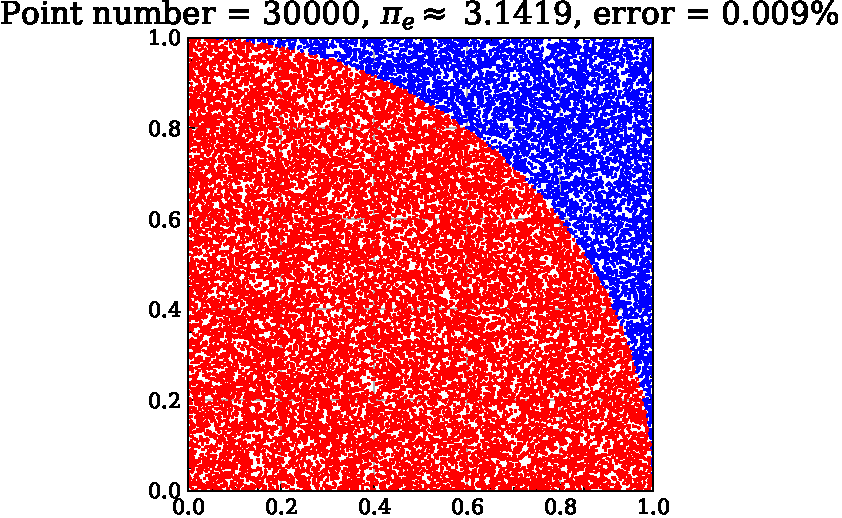
\includegraphics[width=0.7\textwidth]{fig/piEstimation.pdf}\vspace*{-4mm}
\caption{Monte Carlo estimation of $\pi$}\label{fig:Monte Carlo Pi}
\end{figure}

Fig (\ref{fig:Monte Carlo Pi}) illustrates the Monte Carlo simulation result of $N=30000$, and the estimated $\pi_e$ is very close to the real value.

\subsection{Implementation on 2D Ising model}
Consider a $N\times N$ lattice with total particle number $N^2$. Each particle has the spin of $+1$ or $-1$. We can calculate the interaction energy of each particle by the summation of its neighboring four particles, \textit{i.e.}
\begin{equation}
E_{i,j} = -S_{i,j} (S_{i-1, j} + S_{i+1, j} + S_{i, j-1} + S_{i, j+1}) \label{eq:neighboring energy}
\end{equation}

Then we add up all the interaction energy for single particle to get the total energy.

\subsubsection{Initialization}

At first the system can be initialized into a uniform state meaning all the particles have the same spin. From thermal dynamics we know the microscopic state depends on system temperature. The higher the temperature is, the more random the system is. Thus we can throw a random number at one certain temperature $T$ to flip a particle's spin and to see whether the total energy drops or not. Since the total energy is supposed to be minimized, if the total energy of the new state is lower than the older state, the new state is accepted; but if the new energy is higher than the older one, instead of simply rejecting it, we apply the Metropolis method\cite{metropolis}.

\subsubsection{Metropolis method}
When the total energy of the new system is higher than that of the older one (assuming the energy difference is $\Delta E$), we accept it with the probability $e^{-\beta\Delta E = e^{-\frac{\Delta E}{k_BT}}} = e^{-\frac{\Delta E}{T}}$. By ``with the probability of $e^{-\Delta E}$" we mean generating a random number within $[0,1)$ and compare it with $e^{-\Delta E}$; if the generated random number is smaller than $e^{-\Delta E}$ we accept this state.

\subsubsection{Periodic boundary conditions}
We cannot simulate real world crystal as the computation resources for simulation is finite so we must cut off at the edge of the square lattice. The particles inside the square lattice has four interacting neighbor particles, however the particles at the edge have only three or even two neighboring particles. Thus we need to apply periodic boundary conditions (PBC) for boundary particles. When the calculation happens on the boundary particles, we ``borrow'' one or two particles from the opposite border and treat them as the neighboring particles of the boundary particles in order to complete the calculation.

When we have completed all the configurations of the Ising model, we can do the simulation and extract some thermal dynamics parameters from the model, as listed below:
\begin{align}
\braket{E} &= \frac{1}{N^2} \sum\limits_{i} E_i\\
\braket{S} &= \frac{1}{N^2} \ln(\Omega) = \frac{1}{N^2} \ln(\text{C}_{N^2}^{n_{+1}})\\
\braket{C} &= \frac{1}{T^2}\left(\braket{E^2} - \braket{E}^2\right)\\
\braket{M} &= \frac{1}{N^2} \sum\limits_{i} S_i
\end{align}
here the $\Omega$ is the number of possible microscopic states and it can be calculated by the combination number of total particles number and number of spin up particles.

\section{Simulation Results}

Fig (\ref{fig:Results random}) shows the Ising model with a random initial state at different temperature. Noted that at low temperature, the system tend to be aligned at the same direction and several domain emerge. At the critical temperature, the fluctuations of the system is huge and the whole system can no longer remain ordered after iteration. When temperature is high, the system is completely in disordered phase.

\begin{figure}[!h]
\centering
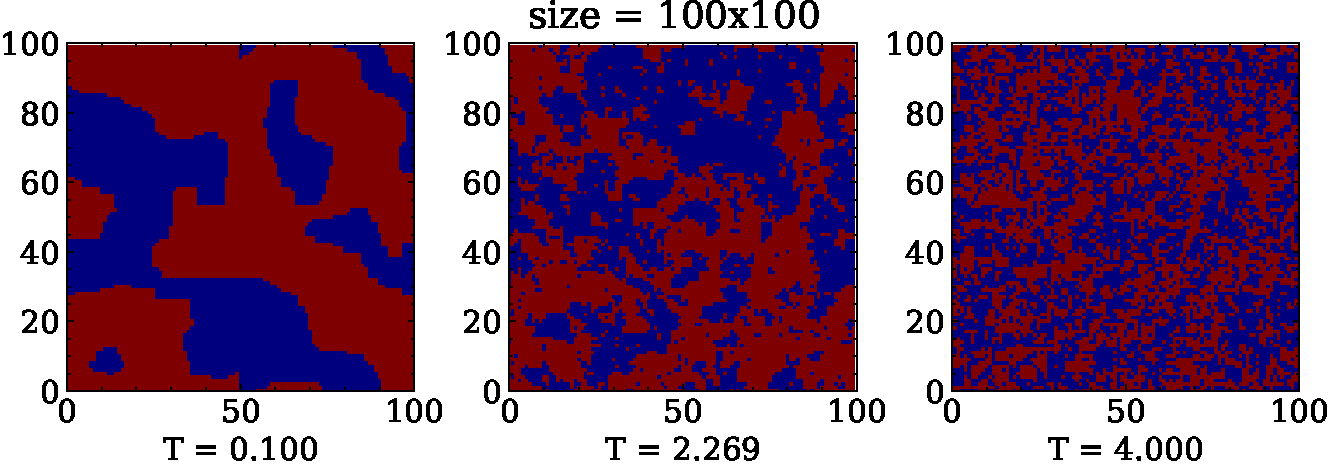
\includegraphics[width=0.9\textwidth]{fig/system-T.pdf}
\caption{Ising model with random initial state}\label{fig:Results random}
\end{figure}

From Fig (\ref{fig:Results uniform}), we can verify the results further. The energy, entropy, specific heat and magnetization are plotted separately. We can see clearly the phase transition happens on the critical temperature $T_c$.

\begin{figure}[!h]
\centering
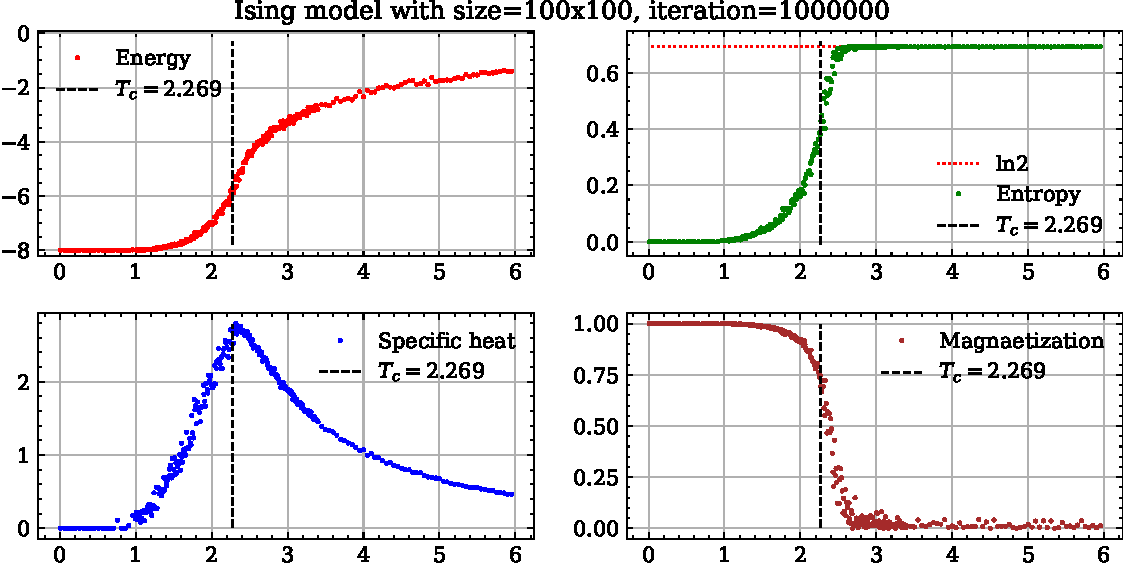
\includegraphics[width=0.98\textwidth]{fig/ESCM-T-size100-iter1000000.pdf}
\vspace*{-4mm}
\caption{Ising model simulation results with uniform initial state}\label{fig:Results uniform}
\end{figure}

%% Bibliography
\newpage
\bibliography{ref}

%% Appendix
\newpage
\appendix
\section{Appendix: Codes}
\subsection{Monte Carlo estimation of $\pi$}
\inputminted[firstline=5,lastline=9]{python}{code/mcpi.py}
\subsection[Monte Carlo simulation of 2D Ising model]{Monte Carlo simulation of 2D Ising model\protect\footnote{This code is updated from this GitHub repo: \url{https://github.com/bdhammel/ising-model}}}
\inputminted[firstline=8,lastline=79]{python}{code/isingTemperature.py}
\subsection{Plotting simulation data}
\inputminted[firstline=6,lastline=24]{python}{code/plotDataFile.py}


\end{document}
